\documentclass[a4paper, 11pt]{article}%тип документа
\usepackage{siunitx}
%отступы
\usepackage[left=2cm,right=2cm,top=2cm,bottom=3cm,bindingoffset=0cm]{geometry}
\usepackage[pdftex]{lscape}
%Русский язык
\usepackage[T2A]{fontenc} %кодировка
\usepackage[utf8]{inputenc} %кодировка исходного кода
\usepackage[english,russian]{babel} %локализация и переносы

%Вставка картинок
\usepackage{wrapfig}
\usepackage{graphicx}
\graphicspath{{Images/}}
\DeclareGraphicsExtensions{.pdf,.png,.jpg}

%Математика
\usepackage{amsmath, amsfonts, amssymb, amsthm, mathtools}

%Заголовокhttps://www.overleaf.com/project/6507f5a4176b25bf05722230
\author{Акимов М.И., Кондратюк Н.А. \\ Б06-206}

\title{Отчёт о выполнении лабораторной работы  \\ \textbf{Адсорбция и мицеллообразование в растворах ПАВ: определение ККМ
по измерению электропроводности и поверхностного натяжения.}}
\date{\\21 февраля 2024 года}
\begin{document}
    \maketitle

       \section{Цели работы.}
        \begin{itemize}
             \item Освоение методик определения критической концентрации мицеллообразования ионогенных и неионогенных ПАВ по измерениям электропроводности и поверхностного натяжения растворов.
             \item Оценка степени ионизации мицелл ионогенных ПАВ по результатам кондуктометрических измерений.
             \item Построение изотермы поверхностного натяжения и адсорбции ПАВ на поверхности раствор/воздух. Определение площади, занимаемой молекулой ПАВ в насыщенном адсорбционном слое.
        \end{itemize}

        \section{Задачи работы.}
         \begin{itemize}
             \item Ознакомиться с содержанием работы; провести необходимые расчёты нужных концентраций ПАВ.
             \item Провести измерения удельной электропроводности растворов ПАВ разных концентраций методом кондуктометрии; провести измерения поверхностного натяжения растворов ПАВ разных концентраций методом пластинки Вильгельми.
             \item Обработать данные, рассчитать требуемые величины (ККМ, степень ионизации и тд.); сравнить полученные значения с теоретическими и табличными.
             \item Сделать выводы о соответствии результатов реальности; сделать выводы о работе в целом; сдать и оформить отчёт о выполнении лабораторной работы.
        \end{itemize}
\newpage
\section{Теоретическое введение.}
\subsection{Кондуктометрический метод.}\,
\par Кондуктометрическое определение ККМ основано на измерении концентрационной зависимости электропроводности растворов ионогенных ПАВ. Измеряя удельную электропроводность при разных концентрациях, можно отметить излом на графике данной зависимости (Рис. 1). Возникает он, естественно, в результате мицеллобразования. 

\begin{wrapfigure}{l}{0.25\textwidth}
    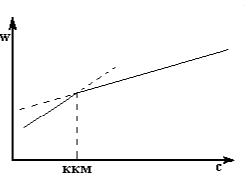
\includegraphics[width=0.25\textwidth]{Images/Fig. 3.png}
    \caption{Зависимость удельной электропроводности раствора ПАВ от его концентрации.}
\end{wrapfigure}\;

\par Объяснить этот эффект можно, во-первых, разностью в подвижности свободных молекул ПАВ и мицелл, а, во-вторых, заряд мицелл может быть сильно меньше суммарного заряда молекул ПАВ в них (из-за степени ионизации).
\par Рассмотрим процесс до достижения ККМ. Согласно уравнению Кольрауша до ККМ удельная электропроводность изменяется по следующему закону:
\begin{equation*}
    \kappa = \lambda_{Na}[Na^{+}] + \lambda_{DS}[DS^{-}]
    \eqno(1.1)
\end{equation*}
\par После достижения ККМ характер зависимости меняется. Для её описания можно рассмотреть процесс только с одной стороны, со стороны изменения заряда мицелл:
\begin{equation*}
    \kappa = \lambda_{Na}[Na^{+}] + \lambda_{DS}[DS^{-}] + \lambda_{mic}[micelle^{-}]
    \eqno(1.2)
\end{equation*}
\par Разрешить это уравнение можно, исходя из следующих предположений:

    $$[DS^{-}] = \text{ККМ}$$
    $$[Na^{+}] = \text{ККМ} + \alpha N [micelle]$$
    $$[micelle^{-}] = \frac{[SDS] - \text{ККМ}}{N}$$
    $$\lambda_{mic} = \alpha N \lambda_{DS}$$
\begin{equation*}
    \kappa = \alpha [SDS] (\lambda_{Na} + \lambda_{DS}) + (1 - \alpha)\text{ККМ}(\lambda_{Na} + \lambda_{DS})
    \eqno(1.3)
\end{equation*}
\subsection{Определение ККМ по изменению поверхностного натяжения раствора ПАВ.}\,
\par Поверхностное натяжение водных растворов ПАВ уменьшается с ростом концентрации вплоть до ККМ (Рис. 2). 

\begin{wrapfigure}{l}{0.25\textwidth}
    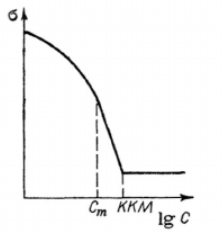
\includegraphics[width=0.25\textwidth]{Images/Fig. 1.png}
    \caption{Изотерма поверхностного натяжения ПАВ.}
\end{wrapfigure} \,

\par Изотерма поверхностного натяжения в
соответствии с уравнением адсорбции Гиббса имеет следующий вид:

\begin{equation*}
    -d\sigma = RT\cdot \text{Г} d\ln(C)
    \eqno(2.1)
\end{equation*}
\par При определенной пороговой концентрации $c_m$ криволинейный участок изотермы переходит в линейный участок с постоянным наклоном, т.е. адсорбция достигает постоянного и максимального значения.
\par При дальнейшем увеличении общей концентрации ПАВ концентрация молекулярного раствора ПАВ перестает расти, в объеме раствора увеличивается концентрация мицелл, и поверхностное натяжение остается практически
постоянным. Величина ККМ определяется по излому изотермы при выходе ее на
горизонтальный участок.

\begin{wrapfigure}{h}{0.25\textwidth}
    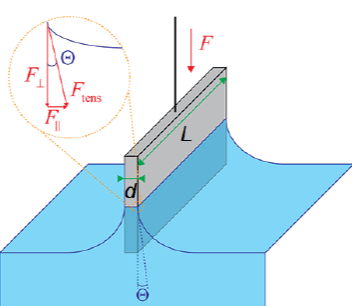
\includegraphics[width=0.25\textwidth]{Images/Fig. 2.png}
    \caption{Cхема определения поверхностного натяжения.}
\end{wrapfigure} \,

\par В данной работе поверхностное натяжение определяется методом пластины
Вильгельми с помощью весов. В раствор с известной концентрацией медленно до касания погружается кусок фильтровальной бумаги. После этого пластинка погружается в раствор на некоторую величину. В итоге на пластинку действуют следующие силы (Рис. 3) 



\par Устройство установки позволяет пренебречь силой Архимеда, а использование фильтровальной бумаги сводит значение $\theta = 0^{\circ}$. В итоге получаем следующее:

\begin{equation*}
\Delta F = 2 \sigma \cdot L
\end{equation*}

\begin{equation*}
\sigma = \frac{m\cdot g}{2L}
\eqno(2.2)
\end{equation*}

\par Полученные из эксперимента данные удобно впоследствии представить в виде графика в полулогарифмических координатах. На графике при этом будет заметен линейный участок изотермы. Аппроксимируя его, можно получить значение предельной адсорбции, используя уравнение Гиббса:
\begin{equation*}
\text{Г}_{\infty} = - \frac{1}{RT}\frac{d\sigma}{d\ln (C)}
\eqno(2.3)
\end{equation*}
\par Из полученного значения легко вычислить площадь, которую приходится на одну молекулу в монослое, и длину углеводородного хвоста молекулы:
\begin{equation*}
S_{0} = \frac{1}{N_{A} \cdot \text{Г}_{\infty}}
\eqno(2.4)
\end{equation*}
\begin{equation*}
l = \frac{\text{Г}_{\infty} \cdot M}{d}
\eqno(2.5)
\end{equation*}
\par Для значений, соответствующих малым концентрациям, применимы предположения адсорбции по Ленгмюру:
\begin{equation*}
\text{Г} = \text{Г}_{\infty} \frac{KC}{KC + 1}
\eqno(2.6)
\end{equation*}
\par Перестроив всё это в линеаризующих координатах, можно вычислить, как значение предельной адсобрции, так и константу равновесия адсорбции:
\begin{equation*}
\frac{1}{\text{Г}} = \frac{1}{\text{Г}_{\infty}} + \frac{1}{KC\text{Г}_{\infty}}
\eqno(2.7)
\end{equation*}
\par По константе из известного соотношения возможно найти стандартную свободную энергию адсорбции:
\begin{equation*}
\Delta G^{\circ} = -RT\ln K
\eqno(2.8)
\end{equation*}
\par Напомним, что из правила Дюкло-Траубе можно рассчитать то же значение, исходя из $\Delta G^{\circ}$ одной $CH_2$ группы.
\newpage
\section{Ход работы.}
\subsection{Кондуктометрия.}
\begin{enumerate}
    \item Все измерения будем проводить с раствором ионогенного ПАВ додецилсульфата натрия (SDS) концентрации $C_{0}$ = 40 мМ. Найдём зависимость электропроводности от концентрации, для этого будем использовать кондуктометр Эксперт-002. Измерительный объём ячейки составляет $V_{0}$ = 22 мл, и чтобы не использовать большое количество посуды с различными разбавлениями, будем использовать метод замещённого объёма. Для этого приготовим первое разведение исходя из стоковой концентрации SDS, а затем будем отбирать объём $V_{i}$ из раствора и добавлять такой же объём стокового раствора (для последовательного концентрирования) или воды (для разбавления). Объём $V_{i}$ определяется следующим образом:
    $$ C_{i+1} = \frac{C_{i}(V_{0}-V_{i})+C_{0}V_{i}}{V_{0}}$$
    $$ V_{i} = {\frac{C_{i+1}-C_{i}}{C_{0}-C_{i}}}V_{0}$$

    \item Согласно формулам выше был расчитан порядок манипуляций для концентрирования (прямого хода) и разведения (обратного хода). При выполнении на каждом этапе  фиксировались показания кондуктометра в режиме термокомпенсации. 

    \begin{table}[h!]
    \centering
    \caption{Результаты измерений электропроводности раствора SDS при изменении концетрации ПАВ (прям. - для последовательного концентрирования, обрат. - для разведения).}
    \begin{tabular}{|l|l|l|l|l|l|}
    \hline
    № & $c, \text{мМ}$ & $V_{i}\text{(прям.)}, \text{мкл}$ & $V_{i}\text{(обрат.)}, \text{мкл}$   &$\kappa \text{(прям.)}, \frac{\text{мкСм}}{\text{см}}$  & $\kappa \text{(обрат.)}, \frac{\text{мкСм}}{\text{см}}$  \\ \hline
    
    1 &	0,82 &	0,451 &	15,603 &	70,65 &	58,7 \\ \hline
    2 &	2,82 &	1,123 &	9,129 &	197,25 & 197,7 \\ \hline
    3 &	4,82 &	1,183 &	6,452	& 315 &	320 \\ \hline
    4 &	6,82 &	1,251 &	3,702	& 406 &	410 \\ \hline
    5 &	8,2	 &  0,915 &	4,4	& 459 &	465 \\ \hline
    6 &	10,25 &	1,418 &	5,6 & 530 &	535 \\ \hline
    7 &	13,75 &	2,588 &	4,464 &	639 &	640 \\ \hline
    8 &	17,25 &	2,933 &	3,711	& 738 &	740 \\ \hline
    9 &	20,75 &	3,385 &	3,443 &	838 &	838 \\ \hline
    10 &	24,6 &	4,4	& & 946 &	946 \\ \hline
    \end{tabular}
    \end{table} 
    \item По полученным данным построим график зависимостии электропроводности от общей концетрации ПАВ для прямого и обратного хода эксперимента(Рис. 4, Рис.5 и Рис.6). 
    \begin{figure}[h!]
	\centering{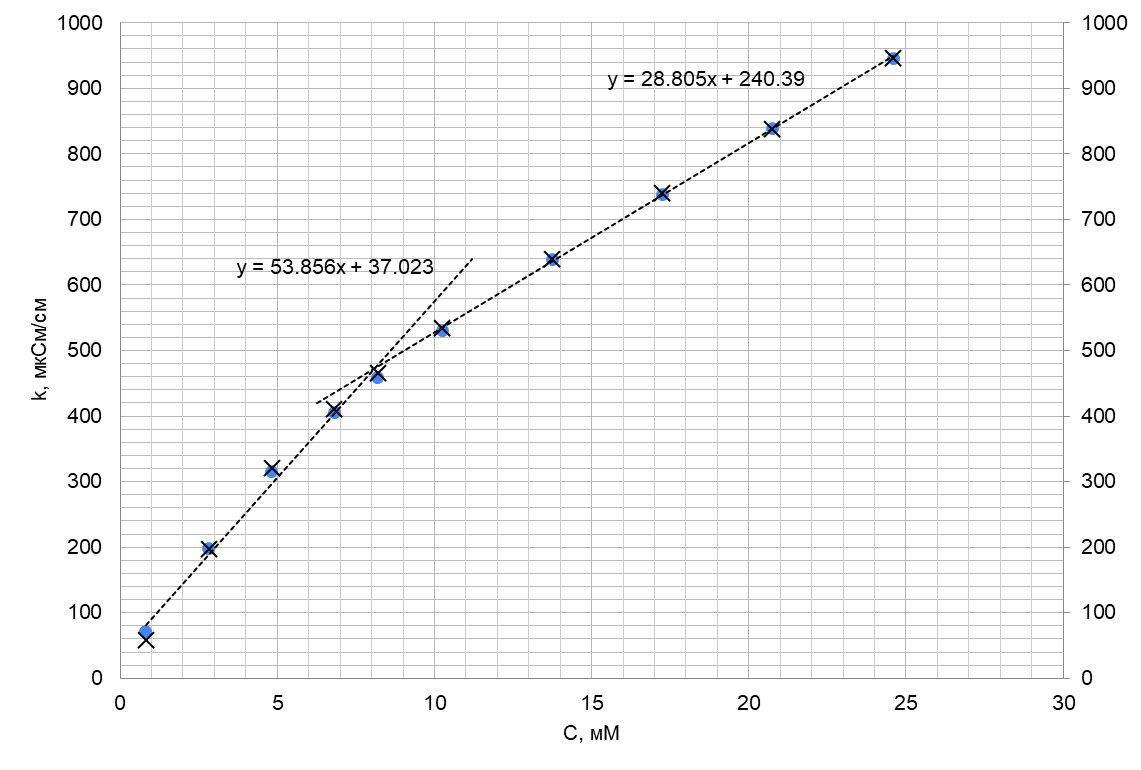
\includegraphics[width=0.8\textwidth]{Images/общий график.jpg}}
        \caption{График зависимости $\kappa(C)$.}
    \end{figure}
    \begin{figure}[!htb]

        \minipage{0.49\textwidth}
            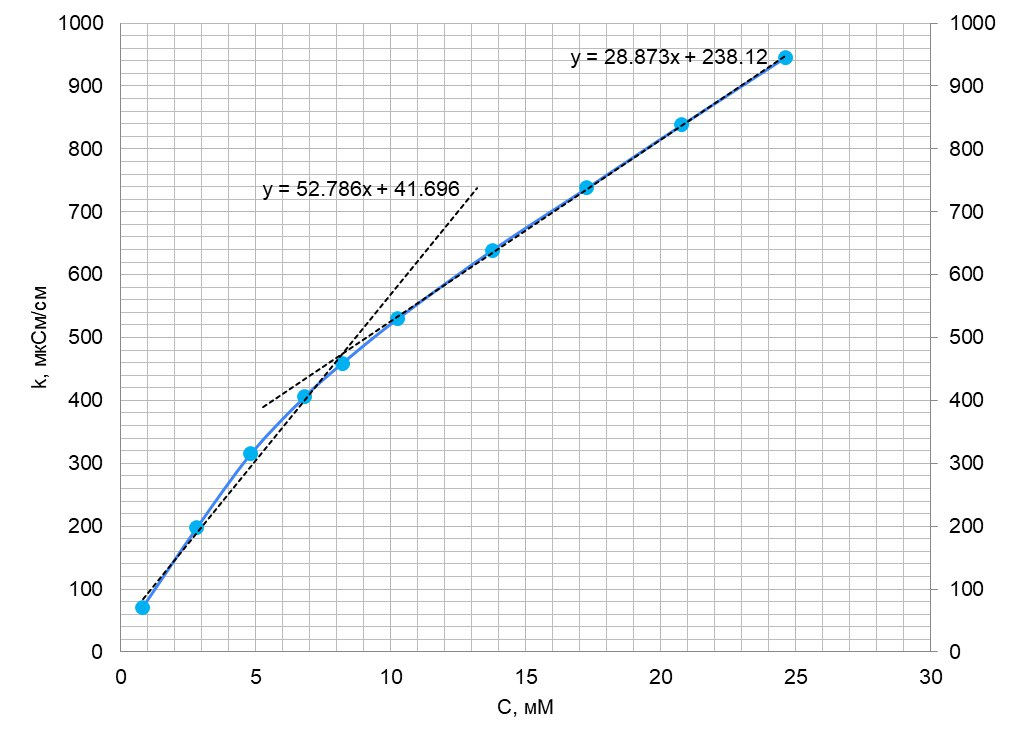
\includegraphics[width=\linewidth]{Images/прямой ход.jpg}
            \caption{График зависимости $\kappa(C)$ при прямом ходе эксперимента }
        \endminipage\hfill
        \minipage{0.49\textwidth}
             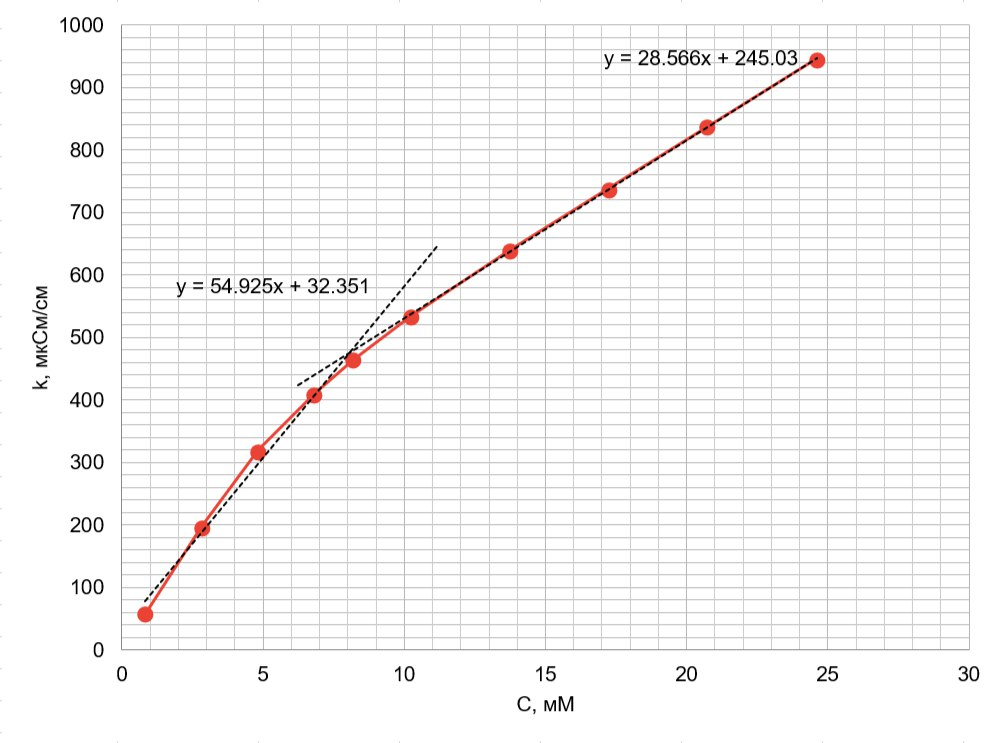
\includegraphics[width=\linewidth]{Images/обратный ход2.jpg}
              \caption{График зависимости $\kappa(C)$ при обратном ходе эксперимента.}
  
        \endminipage
    \end{figure}
    \item По полученным зависимостям определим экспериментальное значение ККМ:
    \begin{table}[h!]
    \centering
    \caption{Экспериментальные значения ККМ}
    \begin{tabular}{|l|l|l|l|}
    \hline
    & Эксперимент  & $\kappa, \frac{\text{мкСм}}{\text{см}}$ &  ККМ, мМ    \\
    \hline
    1& Прямой ход & 475,286 & 8,214   \\
    \hline
    2& Обратный ход  & 475,516 & 8,069  \\
    \hline
    3& Общий график  & 474,232 & 8,118 \\ 
    \hline
    \end{tabular}
    \end{table}
    \item Наиболее точным будет результат для графика прямого хода эксперимента так как ошибки с каждым разведением будут накапливаться, что сказывается на результатах для обратного хода. Так, значение ККМ при повышении концентрации ПАВ совпадает с табличным 8,2 мМ. 
    \item После достижения ККМ наблюдается уменьшение скорости роста электропроводности, так как в растворе уже будут присутствовать и мицеллы, с которыми связано некоторое количество противоионов. Найдём степень ионизации $\alpha$, исходя из изменения угла наклона на графике $\kappa(C)$ (Рис.5).

    Электропроводность до ККМ:
    $$ \kappa_{[SDS] < \text{ККМ}} = (\lambda_{Na}+\lambda_{DS})[SDS] $$
    Электропроводность после ККМ:
    $$ \kappa_{[SDS] > \text{ККМ}} = \alpha (\lambda_{Na}+\lambda_{DS})[SDS] + (1 - \alpha) (\lambda_{Na}+\lambda_{DS})\text{ККМ}$$
    
    Из отношения наклонов получаем степень ионизации $\alpha$ = 54,69\%.
    
\end{enumerate}
\newpage
\subsection{Метод пластинки Вильгельми.}
\begin{enumerate}
    \item Будем проводить измерения, используя раствор додецилсульфата натрия (SDS), пластинку Вильгельми из фильтровальной бумаги (шириной $1$ см и высотой $1,5$ см) и аналитические весы. Для работы подберём 10 точек в диапазоне концентраций от $0,02 \cdot \text{ККМ}$ до ККМ и 3 точки в диапазоне от $1,25 \cdot \text{ККМ}$ до $2,5 \cdot \text{ККМ}$.

    \item Стоит отметить, что длина пластинки может быть далеко от точного значения в $1$ см, так как фильтровальная бумага нарезается в ручную и её длина меняется по мере разбухания. Для этого воспользуемся измерением поверхностного натяжения дистиллированной воды и, сравнив его с табличным, вычислим коэффициент $k$, который в реальности является выражением из следующих величин:
    $$k = \frac{g}{2L}$$
    Получаем:
    $$k \cdot 0,1561 \text{г} = 72,86 \cdot 10^{-3} \frac{\text{H}}{\text{м}}$$
    $$k = 0,467 \frac{1}{\text{с}^2}$$

    \item Произведём серию опытов по определению поверхностного натяжения раствора последовательно каждой концентрации с помощью усреднения максимального значения массы пластинки и вычитания его остаточного веса. По формуле (2.2) вычислим поверхностное натяжение растворов разной концентрации, используя коэффициент $k$ (Таблица 3).

\begin{table}[h!]
\centering
\caption{Результаты измерений поверхностного натяжения SDS.}
\begin{tabular}{|l|l|l|l|l|}
\hline
№ &$C, \text{мМ}$&$m, \text{г}$  &$\sigma, \frac{\text{мН}}{\text{м}}$  & $\ln(C)$  \\ \hline
0   & 0        & 0,1561        &  72,899
&  -infinity
\\ \hline
1   & 0,164        & 0,0976        &  45,579
&  -1,808
\\ \hline
2   & 0,824& 0,0598&  27,927&  -0,194\\ \hline
3   & 0,961        & 0,0561        &  26,175
&  -0,040
\\ \hline
4   & 1,962        & 0,0501        &  23,397
&  0,674
\\ \hline
5& 2,963        & 0,0485        &  22,626
&  1,086
\\ \hline
6& 3,964        & 0,0489        &  22,836
&  1,377
\\ \hline
7& 4,965        & 0,0492        &  22,976
&  1,602
\\ \hline
8& 5,966        & 0,0519        &  24,214
&  1,786
\\ \hline
9& 6,967        & 0,0533        &  24,868
&  1,941
\\ \hline
10& 8,169        & 0,0566        &  26,409
&  2,100
\\ \hline
11& 10,221       & 0,0588        &  27,436
&  2,324
\\ \hline
12& 14,561       & 0,0649        &  30,308
&  2,678
\\ \hline
13& 19,446       & 0,0656        &  30,612
&  2,968\\ \hline
\end{tabular}
\end{table} 
        По полученным данным построим графики зависимости в обычных и полулогарифмических координатах (Рис. 7 и Рис. 8).
\newpage
    \begin{figure}[h!]
	\centering{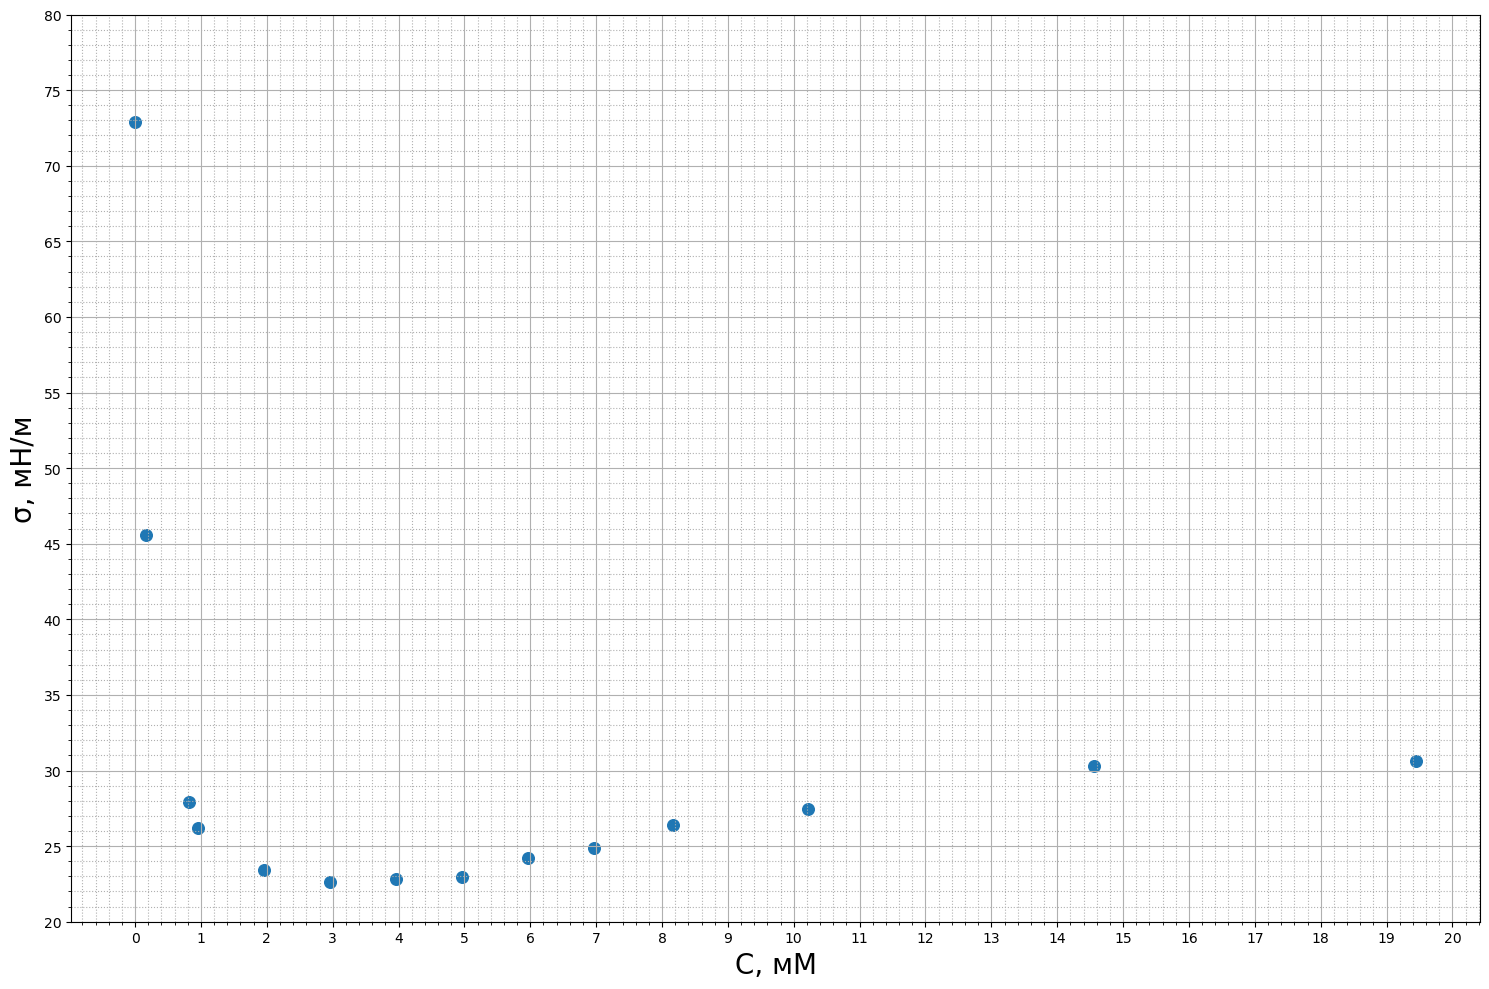
\includegraphics [scale=0.35]{Images/ККМ1.png}}
        \caption{График зависимости $\sigma(C)$.}
    \end{figure}
    \begin{figure}[!htb]

        \minipage{0.5\textwidth}
            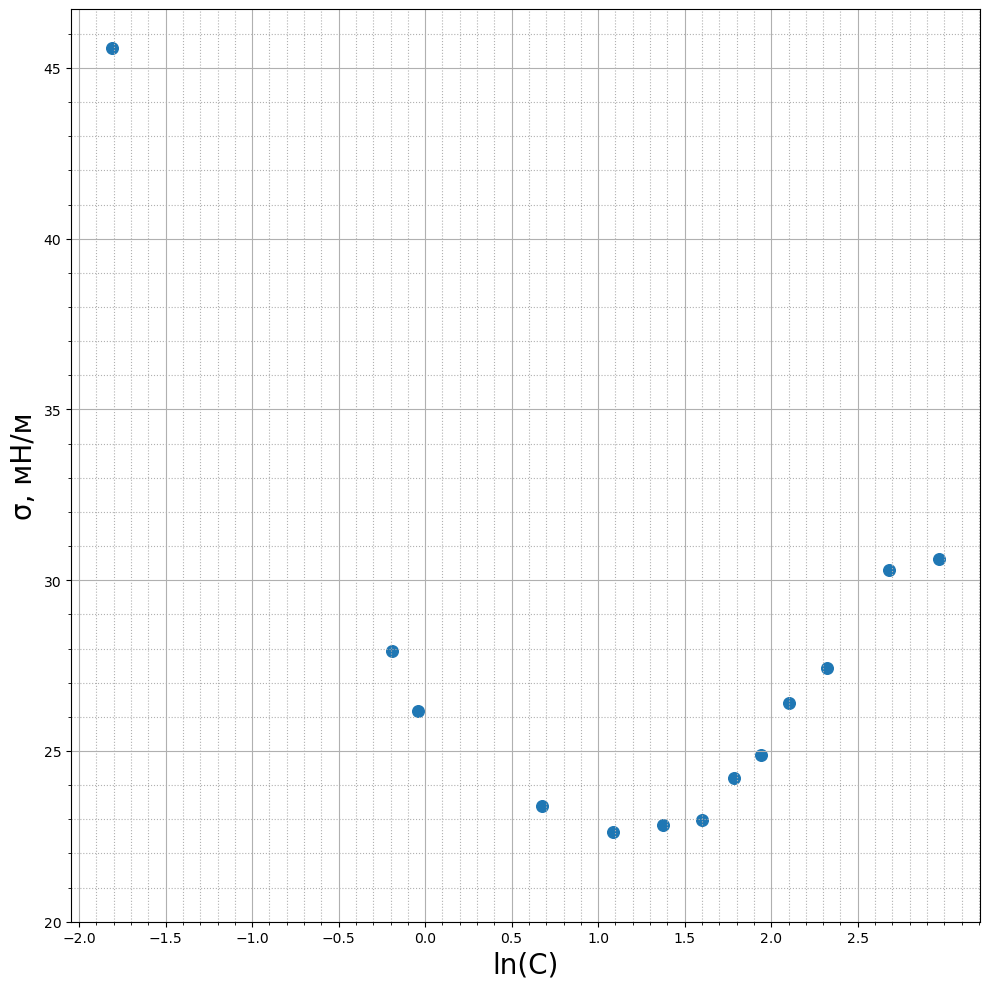
\includegraphics[width=\linewidth]{Images/ККМ2.png}
            \caption{График зависимости $\sigma(\ln(C))$}
        \endminipage\hfill
        \minipage{0.5\textwidth}
             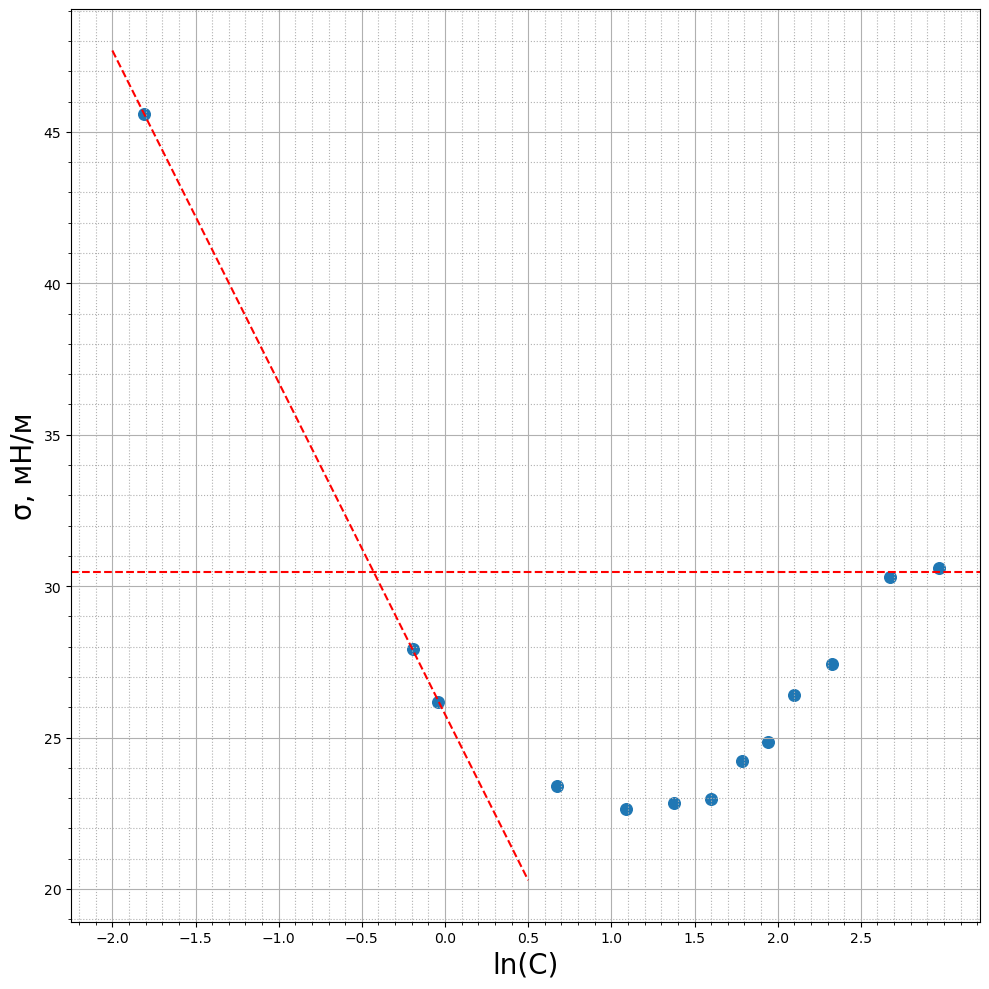
\includegraphics[width=\linewidth]{Images/ККМ3.png}
              \caption{Аппрокимация линейного участка.}
  
        \endminipage
    \end{figure}
        \item По полученным зависимостям можно определить интервал концентраций, в который должен попадать ККМ:
        $$-0,428 \leq \ln(\text{ККМ}) \leq 2,678$$
        $$0,652 \; \text{мМ}\leq \text{ККМ} \leq 14,556\; \text{мМ}$$
        Согласно табличным данным и данным кондуктометрии ККМ в этот диапазон действительно попадает. Однако стоит сказать, что интервал до неприличия большой, что говорит о большой неточности метода пластинки Вильгельми и делает его не пригодным для точного определения ККМ SDS.
        \item На графиках можно заметить минимум значений. Его возникновение обусловлено наличием поверхностно-активных примесей, который понижают поверхностное натяжение раствора даже после достижения ККМ SDS. Рост значений впоследствии является следствием солюбизирующего действия мицелл ПАВ, которые поглощают поверхностно-активные примеси, возвращая поверзностное натяжение к значению, соответсвующему ККМ. Возможные причины возникновения примесей: попадание примесей при приготовлении раствора лаборантами, при взаимодействии со студентами, при транспортировки сухого ПАВ; производство SDS основано на использовании лаурилового спирта, получение которого возможно как синтетически, так и из смеси жиров, что в конечном итоге может привести к большому количеству амфифильных примесей.
        \item Отмечая линейный участок на Рис. 9, определим предельную адсорбцию, используя формулу (2.3). Для этого используем коэффициент наклона линейного участка:
        $$\frac{d\sigma}{d\ln c} = -10,959 \cdot 10^{-3} \,  \frac{\text{Н}}{\text{м}}$$
        Зная, что температура на месте работы составляла примерно $T \approx 294 \, \text{К}$, получим:
        $$\text{Г}_{\infty} = 4,483 \cdot 10^{-6} \; \frac{\text{моль}}{\text{м}^2}$$
        \item По найденной величине адсорбции определим площадь, приходящуюся на одну молекулу в плотном монослое на поверхности раствора по формуле (2.4):
        $$S_{0} = 3,704 \cdot 10^{-19} \; \text{м}^2$$
        \item Задав плотность $d \sim 1 \; \frac{\text{г}}{\text{см}^3}$ адсорбированного ПАВ и зная его молярную массу $M = 288,38 \; \frac{\text{г}}{\text{моль}}$,
        оценим длину молекулы в плотном монослое по формуле (2.5):
        $$l = 1,293 \cdot 10^{-9} \; \text{м}$$
        Для оценки корректности полученного результата, сравним эту величину с
        оценкой по известным геометрическим размерам:
        $$l_{\text{теор}} = 5 \cdot 1,5\sqrt{2(1-\cos(109^{\circ}28^{'}))} + 2 = 14,247 \si{\angstrom} = 1,425 \cdot 10^{-9} \; \text{м}$$
        Как видно из расчётов, экспериментальная величина сходится с теоретической по порядку величины и целому значению. Объяснить этим можно, во-первых, тем, что теоретическая оценка базируется на геометрических приближениях, которые вообще могут быть далеки от реальности. Кроме того, свою погрешность в измерения вносит собственно наличие минимума на кривой, обусловленного поверхностно-активными или гидрофобными примесями.
        \item Аналогично определению предельной адсорбции вычислим величины адсорбции во всех точках изотермы натяжения, посчитав производную с помощью сплайн-интерполяции (Таблица 4).
        \begin{table}[h!]
        \centering
        \caption{Результаты вычисления величины адсорбции до ККМ.}
        \begin{tabular}{|l|l|l|}
        \hline
        № &$C, \text{мМ}$&$\text{Г} \cdot 10^{-6}, \; \frac{\text{моль}}{\text{м}^2}$  \\ \hline
        1 & 0,164        & 4,391 \\ \hline
        2 & 0,824        & 4,639 \\ \hline
        3 & 0,961        & 4,662 \\ \hline
        \end{tabular}
        \end{table}
        Перенесём эти данные на графики (Рис. 10 и Рис. 11)
        \newpage
       \begin{figure}[!htb] 
        \minipage{0.5\textwidth}
            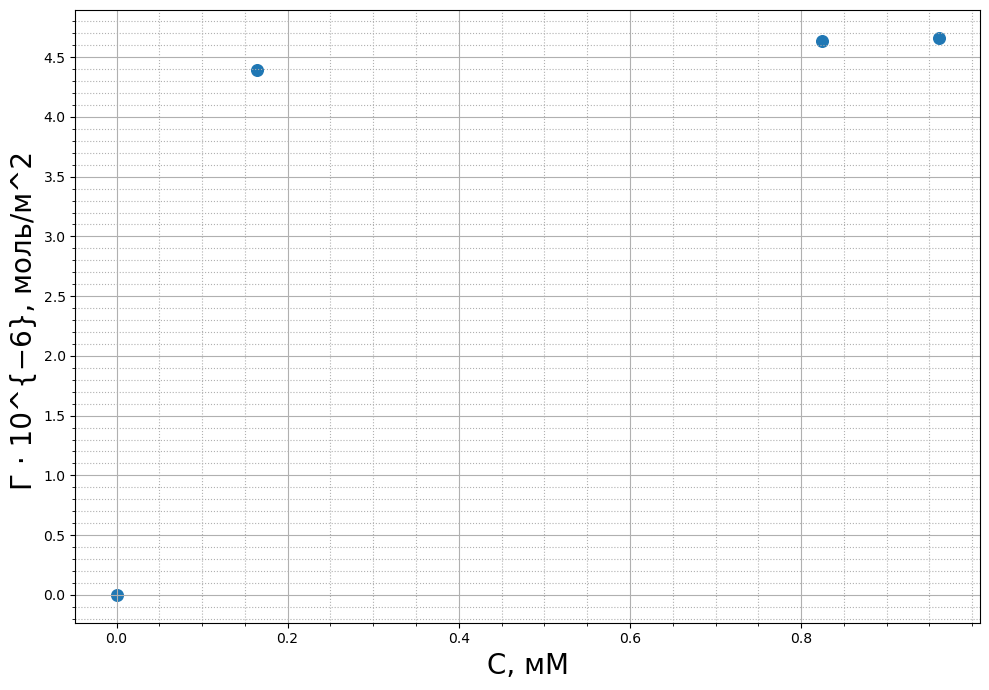
\includegraphics[width=\linewidth]{Images/ККМ4.png}
            \caption{График зависимости $\text{Г}(C)$.}
        \endminipage\hfill
        \minipage{0.5\textwidth}
             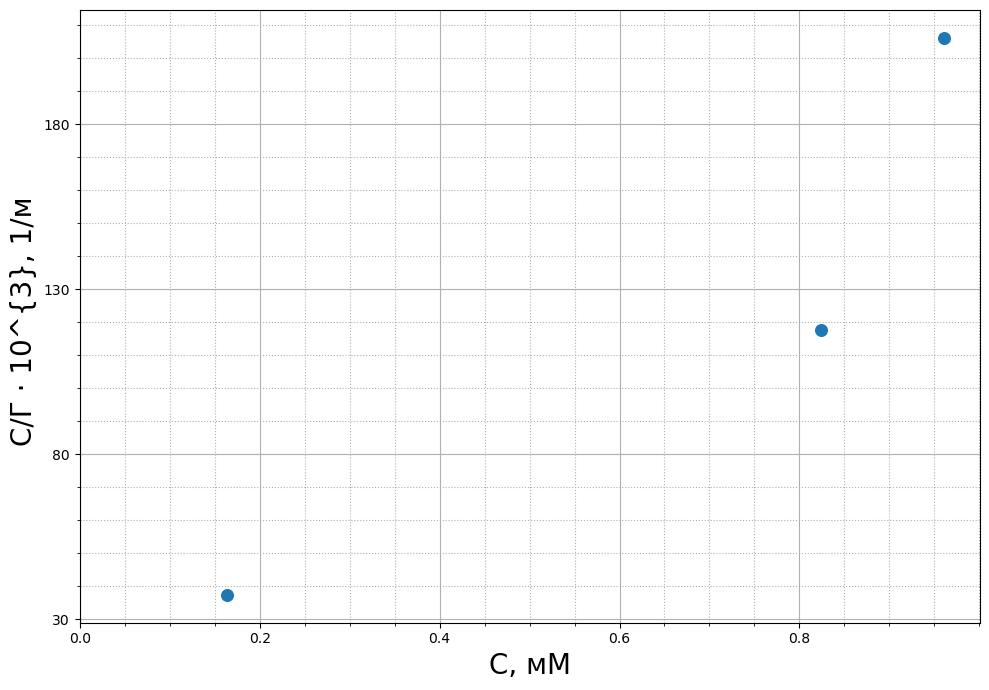
\includegraphics[width=\linewidth]{Images/ККМ5.png}
              \caption{График зависимости $\frac{C}{\text{Г}}(C)$.}
  
        \endminipage
    \end{figure}
    \item Используя формулу (2.7) построим линейную аппроксимацию последнего графика и найдем угловой и свободный коэффициенты (Рис. 12).
    \begin{figure}[h!]
	\centering{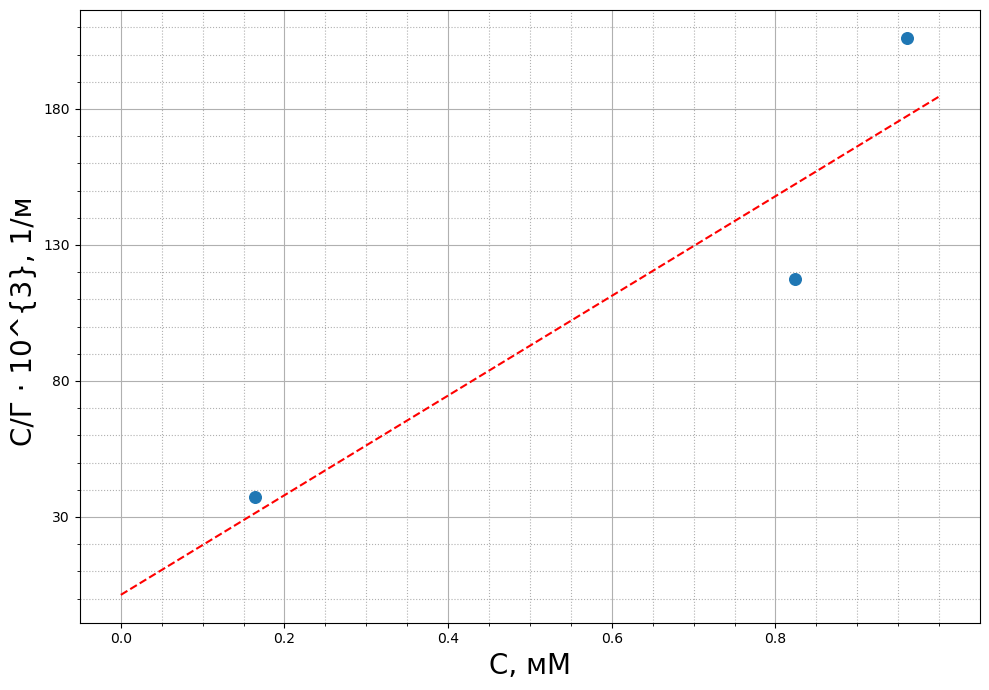
\includegraphics [scale=0.35]{Images/ККМ6.png}}
        \caption{Аппроксимация графика.}
    \end{figure}
    В итоге получаем следующие значения:
    $$\frac{1}{\text{Г}_{\infty}} = 183,218 \cdot 10^{3} \; \frac{\text{м}^2}{\text{моль}}$$
    $$\frac{1}{K\text{Г}_{\infty}} = 1,339 \cdot 10^{3} \; \frac{\text{м}^2}{\text{моль}}$$
    Из этих значений получим значения предельной адсорбции и константы мицеллообразования:
    $$\text{Г}_{\infty} = 5,458 \cdot 10^{-6} \; \frac{\text{моль}}{\text{м}^2}$$
    $$K = 136,831 \cdot 10^{3}\; \frac{1}{\text{М}}$$
    Видно, что по порядку величины данное значение сходится с найденным ранее. Однако, хочется отметить, что при аппроксимации по двум точкам (запрещено на территории МФТИ) значение абсолютно совпадает с найденным из изотермы поверхностного натяжения. 
    \item По формуле (2.8) найдём $\Delta G^{\circ}$:
    $$\Delta G^{\circ} = - 28,908 \; \text{кДж}/\text{моль}$$
    Теоретическое значение посчитаем по правилу Дюкло-Траубе:
    $$\Delta G^{\circ}_{\text{теор}} = - 22,08 \; \text{кДж}/\text{моль}$$
    Таким образом, теоретическое и экспериментальное значения не совпадают уже по второму целому числу. Однако стоит учитывать, что теоретическое значение посчитано приближённо, а экспериментальное имеет большую погрешность по ряду причин. 
  \end{enumerate}
\section{Выводы.}

\begin{itemize}
    \item В первой части работы с помощью кондуктометрического метода была установлена зависимость удельной электропроводности от концетрации ионногенного ПАВ SDS (для приготовления растворов разной концетрации использовался метод замещённого объёма). В точке излома было определено эксперементальное значение ККМ, которое совпало с табличным (8,2 мМ). Также, по изменению угла наклона графика $\kappa(C)$ определили степень ионизации мицелл SDS ($\alpha$ = 54,69\%).
    \item Для исследования зависимости поверхностного натяжения от концентрации ПАВ был использован метод пластинки Вильгельми. В результате были получены данные, позволяющие грубо оценить диапазон значений ККМ (данный эффект обуславливается наличием поверхностно-активных и гидрофобных примесей в растворе). По линейному участку данной зависимости, представленной в полулогарифмических координатах, было определено значение предельной адсорбции  $\text{Г}_{\infty} = 4,483 \cdot 10^{-6} \; \frac{\text{моль}}{\text{м}^2}$, а из него величины площади $S_{0} = 3,704 \cdot 10^{-19} \; \text{м}^2$ и длины $l = 1,293 \cdot 10^{-9} \; \text{м}$ (совпадает с теоретической по порядку и целому значению) одной молекулы ПАВ в монослое. Путём построения зависимости адсорбции от концентрации была посчитана константа мицеллобразования $K = 136,831 \cdot 10^{3}\; \frac{1}{\text{М}}$ и стандартная свободная энергия Гиббса адсорбции SDS $\Delta G^{\circ} = - 28,908 \; \text{кДж}/\text{моль}$ (совпадает с теоретической по порядку величины).  
\end{itemize}

\end{document}